\documentclass{IEEEtran}
%\textwidth 6.8in \addtolength{\oddsidemargin}{-1.1in}
%\textheight 10in
%\addtolength{\topmargin}{-0.5in}
%\setlength{\parindent}{0.0cm}
%\setlength{\parskip}{0.1cm}
%\topskip 0.0in

\author{Siddharth Goyal 15UCS140 | Kanak Singhal 15UCS057}
\title{Report on IT Workshop Project}

\usepackage{amsmath}
\usepackage{graphicx}

\begin{document}
\maketitle

%\begin{center}
%This is how to put text in center of thw qwdasdasfsfdsfds dsgdsgdsf
%\end{center}

\section{Introduction}
\label{sec:intro}
The project outlines the analysis of the various algorithms used to sort arrays. This is of particular importance is handling large amount of data. An efficient algorithm gives better results for the organiser. Use of LaTeX and GNUplot has been extensive in the project to facilitate it.

\section{Algorithm analyzed}
\label{sec:algo}

The following algorithms have been analyzed:-
\begin{itemize}
\item Bubble Sort
\item Insertion Sort
\item Merge Sort
\item Quick Sort
\item Selection Sort
\end{itemize}
%\label{sec: enumerate}
%\subsection{Enumerate}
%\begin{enumerate}
%\item first bullet
%\item second bullet
%\end{enumerate}

\section{Method of analysis}
\label{sec: method}
%of almost $\infty$ (the set of available fonts are huge)
%fonts, you can use greek leeters or any other simple by using a \textbackslash ~~~$\alpha$, \[beta\] and $\gamma$.\\
%%$f(x)=x^25
%${f(x) = x^2}
To analyze the varios algorthms we have generated a random array of numbers. The arrays are varied in size to compute the working of algorithms in various environments. The same array is sorted using all the algorithms and the number of comparisions are calculated. The algorithm with the most comparisons is the least efficient. Time taken by different algorithms to sort the given data is also considered.
This is indeed a good measure of performance, especially since it’s independent of the underlying hardware design.
%\subsection( this is how you write equations and label them )

\section{Analysis of algorithms}
\label{sec:anal}
\subsection{Bubble Sort}
Bubble sort algorithm, also referred to as sinking sort algorithm, is a simple sorting algorithm. The algorithm sorts the given array by fixing from the first unit and then comparing the array in adjacent pairs from the last, it swaps the pair if it is in wrong order. Then the algorithm repeats itself for every element in the array except the last one. This continuous process sorts all the elemets in the desired order. The algorithm, which is a comparison sort, is named for the way smaller elements "bubble" to the top of the list. \\
\textbf{\underline{Best case}}: \[n^2\]
\textbf{\underline{Average case}}: \[n^2\] 
\textbf{\underline{Worst case}}:\[n\]

\subsection{Insertion Sort}
Insertion sort algorithm is a simple sorting algorithm. The algorithm works by fixing on the second element from the start and then comparing the preceeding elements. The preceeding elements are sorted by comparing them in pairs and are swapped if necessary. Otherwise the point is replaced by the current temp value in the loop, This repeats for all the succeeding elements in the array.\\
\textbf{\underline{Best case}}: \[n^2\]
\textbf{\underline{Average case}}: \[n^2\] 
\textbf{\underline{Worst case}}:\[n\]  

%\subsection{Merge Sort}
%Merge sort is a very efficient algorithm. Merge sort is a divide-and-conquer algorithm. The unsorted array is divided into sub-parts which are further divided till individual elements remain. The individual elements are compared and merged into sections which are further compared and merged. The final merge gives a sorted array. For large n and a randomly ordered input list, merge sort's expected (average) number of comparisons approaches α·n fewer than the worst case where 
%\begin{align}
%\alpha=\displaystyle\sum\limits_{k=0}^\infty\frac{1}{2^k + 1} \approx 0.2645 
%\end{align}
%\textbf{\underline{Best case}}: \[n log n\]
%\textbf{\underline{Average case}}: \[n log n\] 
%\textbf{\underline{Worst case}}:\[n\]

\subsection{Quick Sort}
Quicksort also called as partion-exchange sort is an efficient sorting algorithm, serving as a systematic method for placing the elements of an array in order. Analysis of quicksort shows that, on average, the algorithm takes O(n log n) comparisons to sort n items. In the worst case, it makes O(n2) comparisons, though this behavior is rare. The worst case of the quicksort algorithm only occurs when the pivot choosen is the biggest or the smallest element in the array.\\
\textbf{\underline{Best case}}: \[n log n\]
\textbf{\underline{Average case}}: \[n log n\] 
\textbf{\underline{Worst case}}:\[log n\]

\subsection{Selection sort}
Selection sort is a simple sorting algorithm. The process itself is very simple. The first element is taken as base, relative to which the array is scanned. When an element smaller than base comes up that element is made as base and the scanning continues. Then it is swapped with the first element. Now the same process is repeated from the second element till the (n-1) element. Although it is very inefficient in conventional sense due to high number of comparisions involved, the seletion sort is very simple to understand and use.\\
\textbf{\underline{Best case}}: \[n^2\]
\textbf{\underline{Average case}}: \[n^2\] 
\textbf{\underline{Worst case}}:\[n^2\]

\section{GNU Plots}
\label{sec: plot}
\textbf{GNU Plot of Number of comparisions and size of arrays}
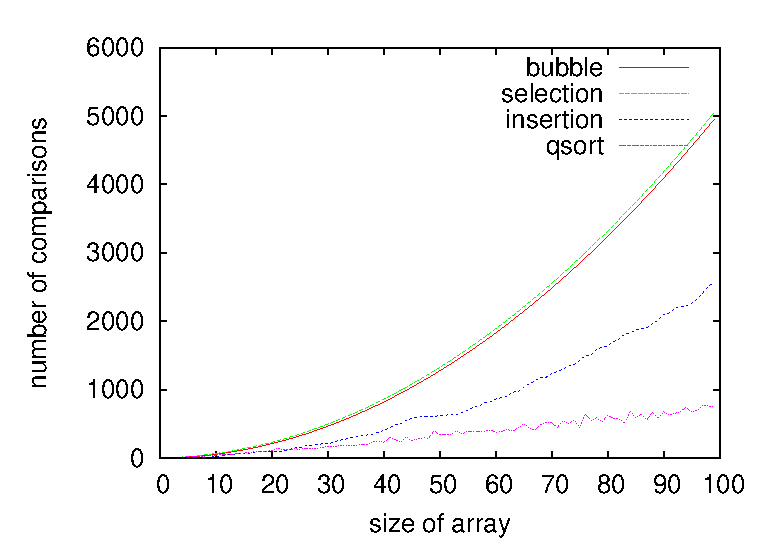
\includegraphics[scale=0.75]{noc.eps}
\textbf{GNU Plot of execution of time and size of arrays}
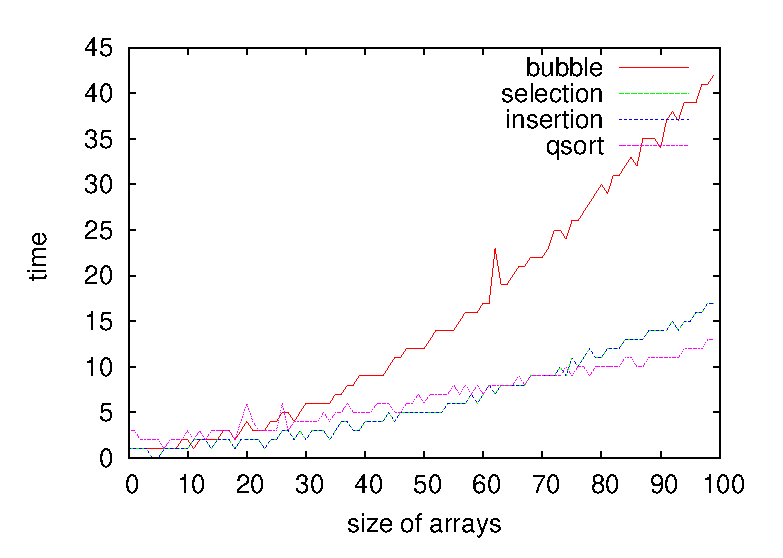
\includegraphics[scale=0.75]{time.eps}


\section{Conclusion}
\label{sec:conc}
The analysis of the above algorithms gives us that divide-and-conquer algorithms like Merge sort and Quick sort are faster and more efficient. Taking the random data into account we can conclude the following:-  
\begin{itemize}
\item Selection sort is the worst algorithm to sort data even more than Bubble sort by the GNU plots.
\item Quicksort is the best algorithms to sort an array when the pivot is taken randomly for a completely random data set.
\end{itemize}

%\begs5\,^{\circ}\mathrm{c}$
%\\ \hline

%\end{tabular*}
%\end{center}
%\end{table}

%For Introduction goto section \ref{sec:intro} \\
%For Algorithm analyzed goto section \ref{sec:algo}\\
%For Method of analysis \ref{sec: method}\\
%For Analysis of algorithms\ref{sec:anal}\\
%For GNU Plots\ref{sec: plot}\\
%For Conclusion\ref{sec:conc}






%\bibliographystyle{IEEEtran}
%\bibliography{goyal}
%\cite{erdos1935difference}


\end{document}

